% Insert into a Chinese-capable LaTeX document (for example, XeLaTeX + ctex).
% Compile with the manuscript directory as the working directory.
\begin{figure*}[t]
  \centering
  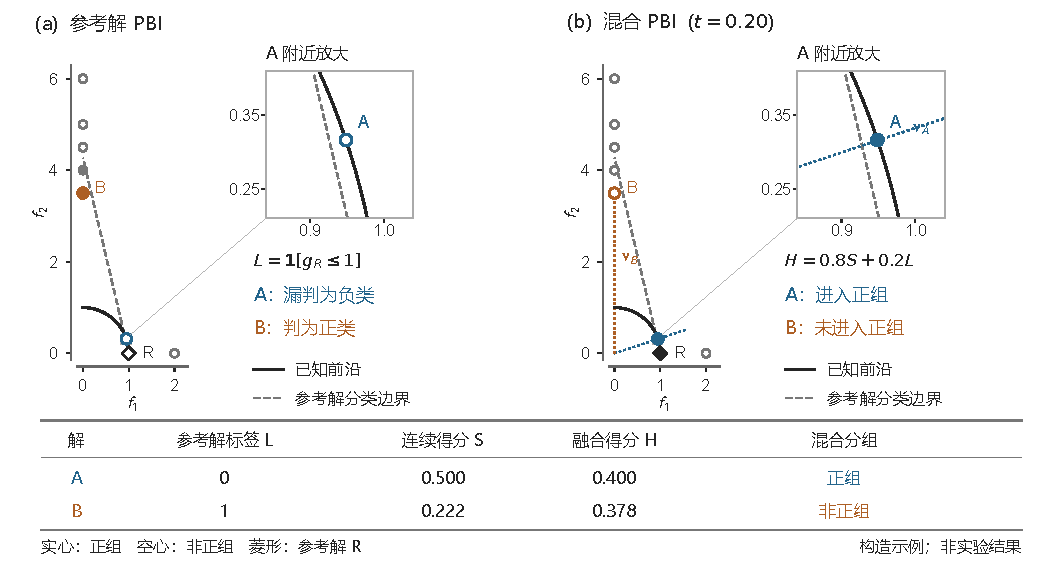
\includegraphics[width=180mm]{figures/paqc_correction_example/paqc_correction_cn.pdf}
  \caption{方向信息对参考解 PBI 分组的修正示例。
  两幅图采用同一组八个构造目标向量，考虑
  $f_1,f_2\geq0$、$f_1^2+f_2^2\geq1$ 上的二维最小化问题。
  单位圆弧为已知 Pareto 前沿，仅用于评价图中判定，不参与两种方法的评分。
  (a)~给定参考解 $R=(1,0)$ 和 $\delta=0.234375$，参考解分类得到
  $L_A=0$、$L_B=1$，其中 $A=(3/\sqrt{10},1/\sqrt{10})$ 位于前沿，
  $B=(0,3.5)$ 位于前沿外侧。虚线为计算得到的参考解分类边界。
  (b)~取 $\theta=5$、预算进度 $t=0.20$，按 $H=0.8S+0.2L$ 融合，
  八个解中排名前两位的 $A$、$R$ 进入正组，$B$ 未入选。
  点线表示 $A$、$B$ 关联的参考方向；相同范围的放大窗显示 $A$ 附近的判定变化。
  实心与空心分别表示进入和未进入对应正组，菱形表示参考解。
  下表给出关键解的实际计算得分。标签遵循当前数值实现，包括其对分类边界点的处理。
  本图是给定参考解与参数的分类机制示例，不是实验结果，也不验证参考解选择过程；
  所示修正发生在预算早期，不能推广为整个预算阶段均能跨标签纠错。}
  \label{fig:paqc-correction-example-cn}
\end{figure*}
